When you apply the polygon-union algorithm from \hyperref[blogpart1]{part 1},
you face a challenging question: What should we do if we find polygons that have
similar colors and these colors are different? Kopf-Lischinski paper don't
explore this issue at all and the results from their
\href{http://research.microsoft.com/en-us/um/people/kopf/pixelart/supplementary/index.html}{supplementary
material} show random results (sometimes the color information is simply lost
and sometimes they are preserved and smoothed by the rendering technique
chosen).

libdepixelize's approach is to preserve as much color information as possible
and this approach led to some extensions to the algorithm (with more to come).
The first rule is:

\begin{equation}
  \label{ec:foundation}
  \text{\textbf{Don't discard color information\ldots ever}!}
\end{equation}

The effect of the rule \ref{ec:foundation} is that only polygons of the same
color should be united together.

But if I don't discard color information, the splines will become visually
disconnected. What should I do? First, let's review the node types with the
following image:

\begin{figure}[H]
  \centering
  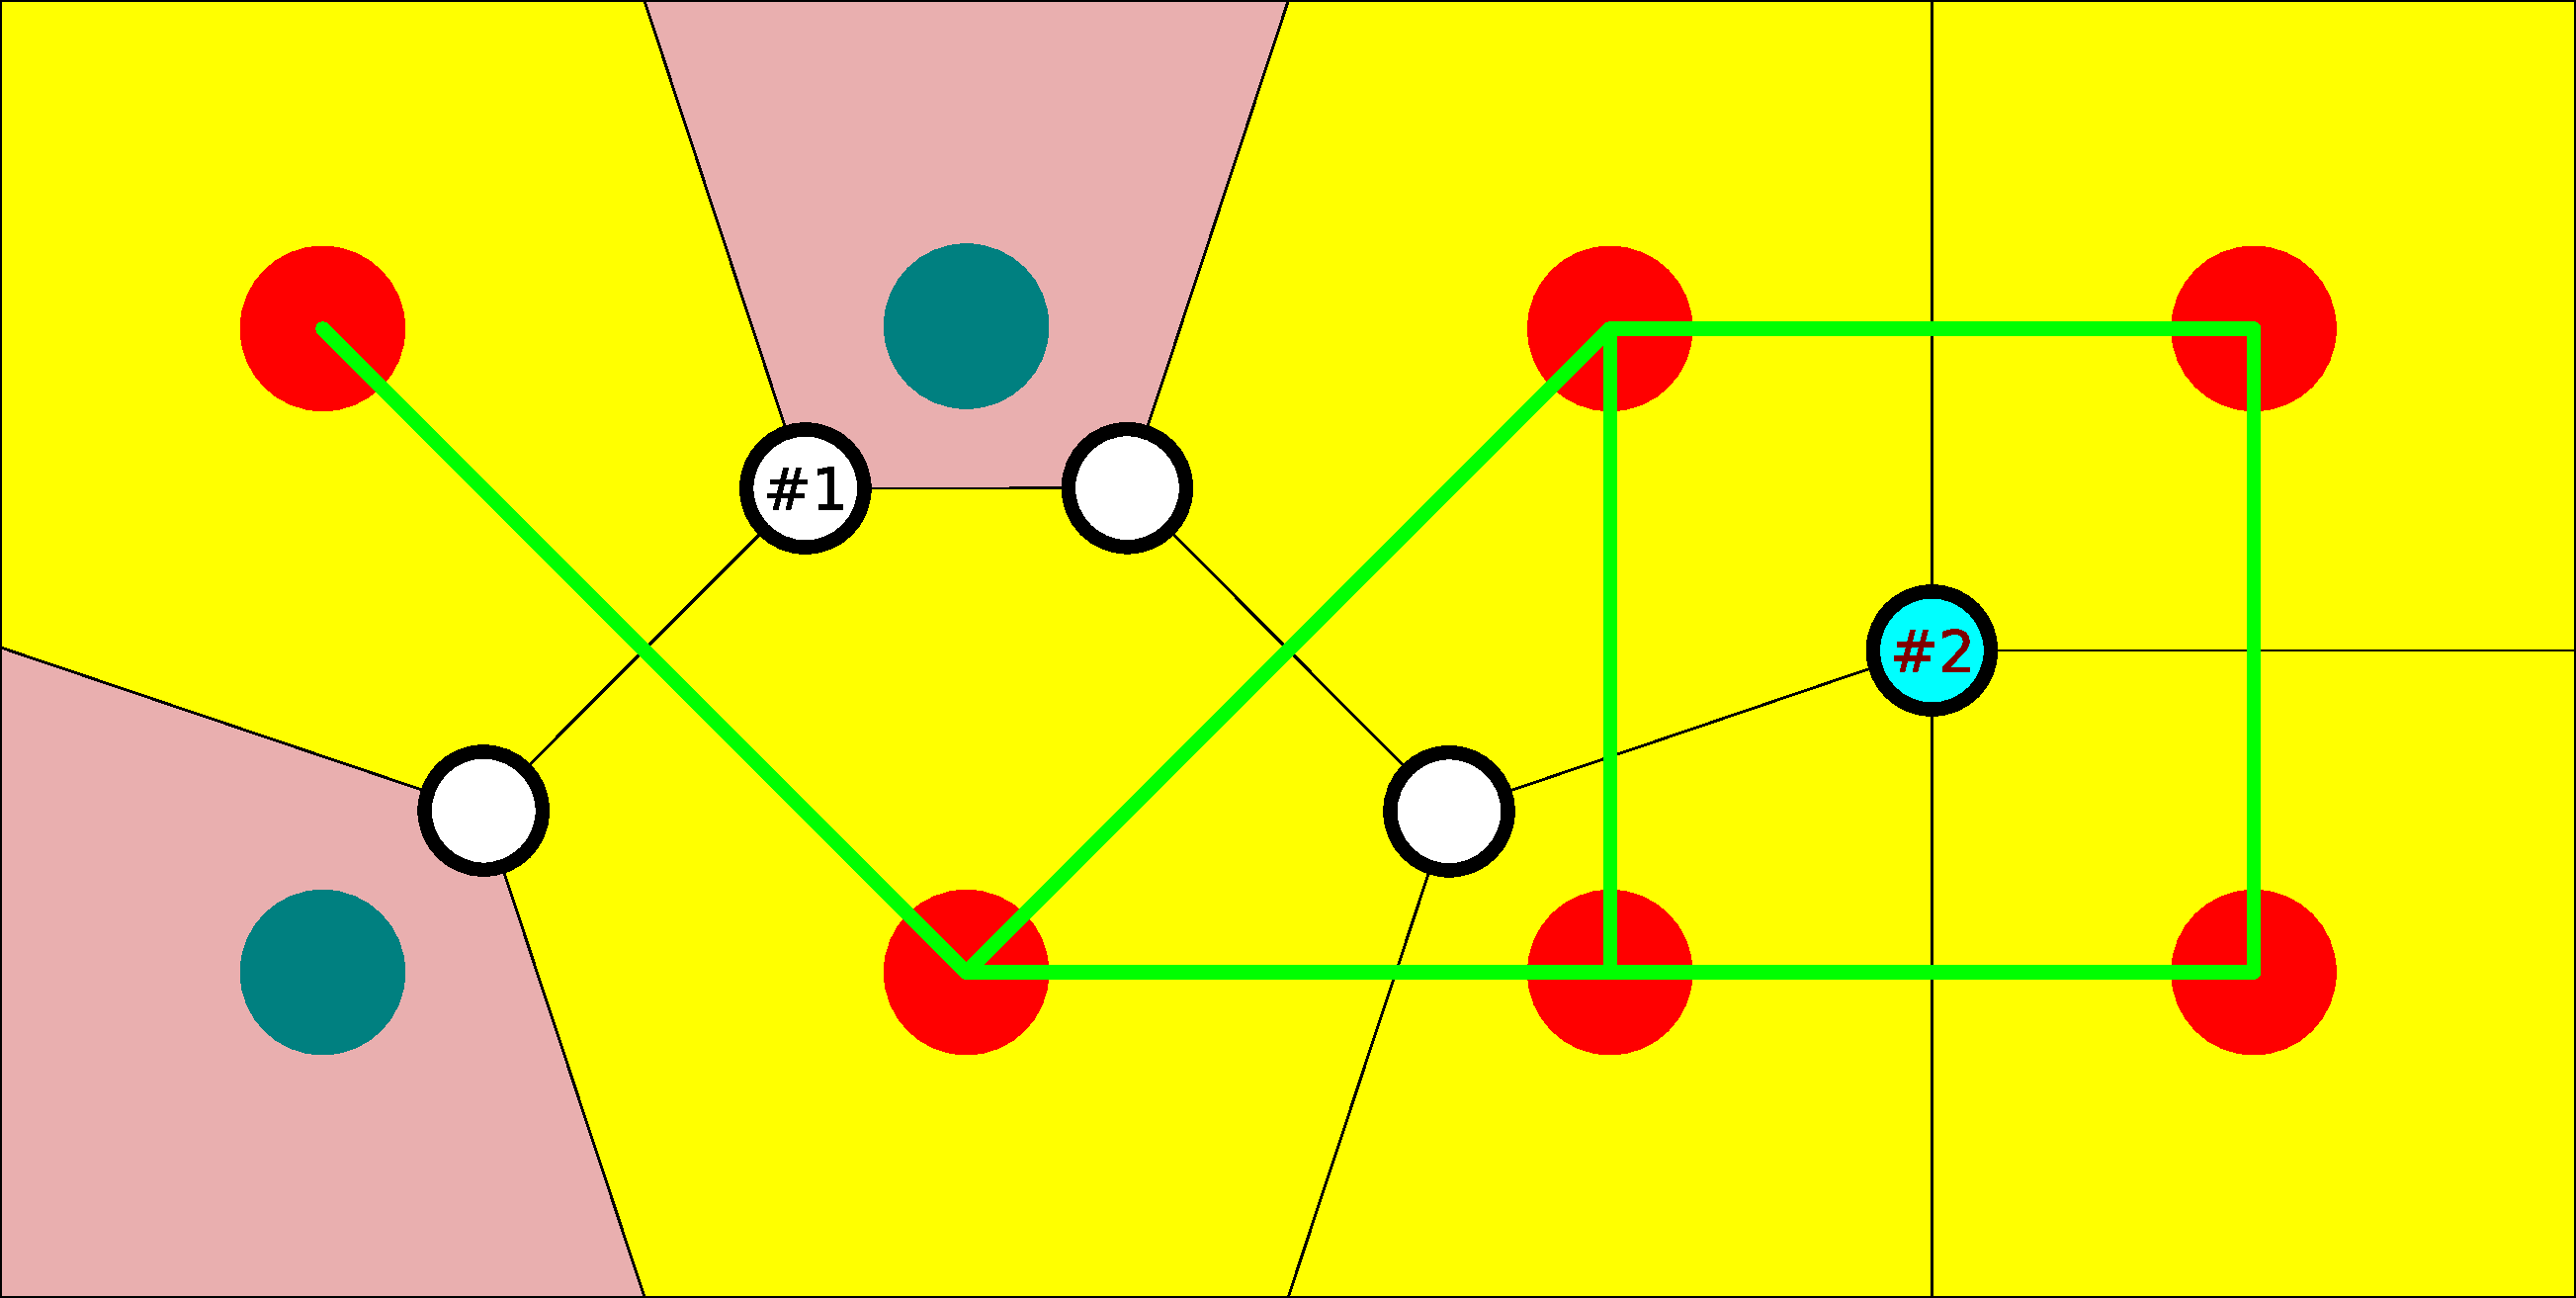
\includegraphics[width=0.8\textwidth]{assets/voronoi3.pdf}
  \caption{Vertex types}
\end{figure}

There are special heuristics about what to do for each node type and these
heuristics are organized in some sections below.

Another interesting figure to introduce is the \emph{boof} character.
\emph{Boof} has a color palette and pixel patterns that help to explain the
heuristics responsible for extra color information. The Voronoi diagram
generated by boof input is shown below.

\begin{figure}[H]
  \centering
  
\includegraphics[width=0.8\textwidth]{assets/boof_voronoi.pdf}
  \caption{\emph{Boof}, kindly created by Jabiertxo Arraiza Cenoz and
    ``licensed'' under public domain (CC0).}
\end{figure}

\section{Cyan (\#2) nodes}
\label{cyan_nodes}

If you find a node for which the surrounding cells have similar colors, but not
equal, then you check if the colors of both sides of an edge are equal. There
are four edges and the node will be smooth if the total number of ``equal
colors'' counts two.

The following picture highlight the separating edges you need to check.

\begin{figure}[H]
  \centering
  
\includegraphics[width=0.8\textwidth]{assets/boof_cyan.pdf}
  \caption{Cyan node where the interesting separating edges are highlighted in
    green.}
\end{figure}

The result of this heuristic for the previous picture follows:

\begin{figure}[H]
  \centering
  
\includegraphics[width=0.8\textwidth]{assets/boof_cyan2.pdf}
  \caption{Cyan node highlighted with a green circle.}
\end{figure}

\subsection{Why does it work?}

We have a heuristic and its results are quite good, but maybe you're
wondering\ldots why does it work?

First requirement for \emph{some} of these heuristics work is:

\begin{equation}
  \label{ec:same answer}
  \text{The answer must be the same for all nodes sharing the same position.}
\end{equation}

And our heuristic fulfill the requirement \ref{ec:same answer}, because it uses
the same local data for all four nodes sharing the same position.

If a heuristic don't fulfill the requirement \ref{ec:same answer}, then it
should have extra effects such as ``adjust B-Spline'' to produce good results.

The other requirement for a good heuristic is:

\begin{equation}
  \label{ec:visually connected}
  \text{The result shouldn't create distant or overlapping segments.}
\end{equation}

And this heuristic fulfill the requirement \ref{ec:visually connected} too,
because it only creates smooth nodes when three cells are going to be grouped.
If three cells of the four will be grouped, then the result will be two large
polygons. When the region affected by the smooth node is shared by two polygons
only, the two will perfectly complete each other.

\section{White (\#1) nodes}
\label{white_nodes}

\begin{figure}[H]
  \centering
  
\includegraphics[width=0.8\textwidth]{assets/boof_white.pdf}
  \caption{White node with the borders/edges highlighted in green.}
\end{figure}

For this type of node, we know in advance that two of the cells surrounding it
have similar colors and we will refer to them as the \emph{twin cells}. We will
refer to the other cell as the \emph{third cell}.

The node within the \emph{third cell} will always be smooth.

The nodes within the \emph{twin cells} will be smooth \textbf{if} any two of the
three cells have the same color. If the node is \textbf{not} smooth, then it
needs to be properly adjusted using the technique from
\hyperref[tjunction]{T-junctions section} to properly lie on the smooth curve
affected by the \emph{third cell}.

You can see some examples of this heuristic below:

\begin{figure}[H]
  \centering
  
\includegraphics[width=0.8\textwidth]{assets/boof_white2.pdf}
  \caption{White node heuristic producing a non-smooth node.}
\end{figure}

This heuristic doesn't fulfill requirement \ref{ec:same answer}, but it will
produce a good result thanks to the special handling of non-smooth nodes using
the trick from \hyperref[tjunction]{T-junctions section}.

\begin{figure}[H]
  \centering
  
\includegraphics[width=0.8\textwidth]{assets/boof_white3.pdf}
  \caption{White node heuristic producing a smooth node.}
\end{figure}

\section{The evil pattern}

Thanks to the rule \ref{ec:foundation}, we lose the transitivity property. The
lack of transitivity introduces some unusual patterns that I refer to as an
\emph{evil pattern}. I identified some evil patterns.

\subsection{The evil pattern \#1}

An example of the \emph{evil pattern \#1} follows:

\begin{figure}[H]
  \centering
  
\includegraphics[width=0.8\textwidth]{assets/evil_pattern.pdf}
  \caption{An evil pattern. A green line represents a connection (based on the
    similarity graph).}
\end{figure}

We handle the \emph{evil pattern \#1} using the rules for the
\hyperref[cyan_nodes]{cyan nodes}. This pattern doesn't generate extra
complication.

\subsection{The evil pattern \#2}
\label{evil_pattern2}

An example of the \emph{evil pattern \#2} follows:

\begin{figure}[H]
  \centering
  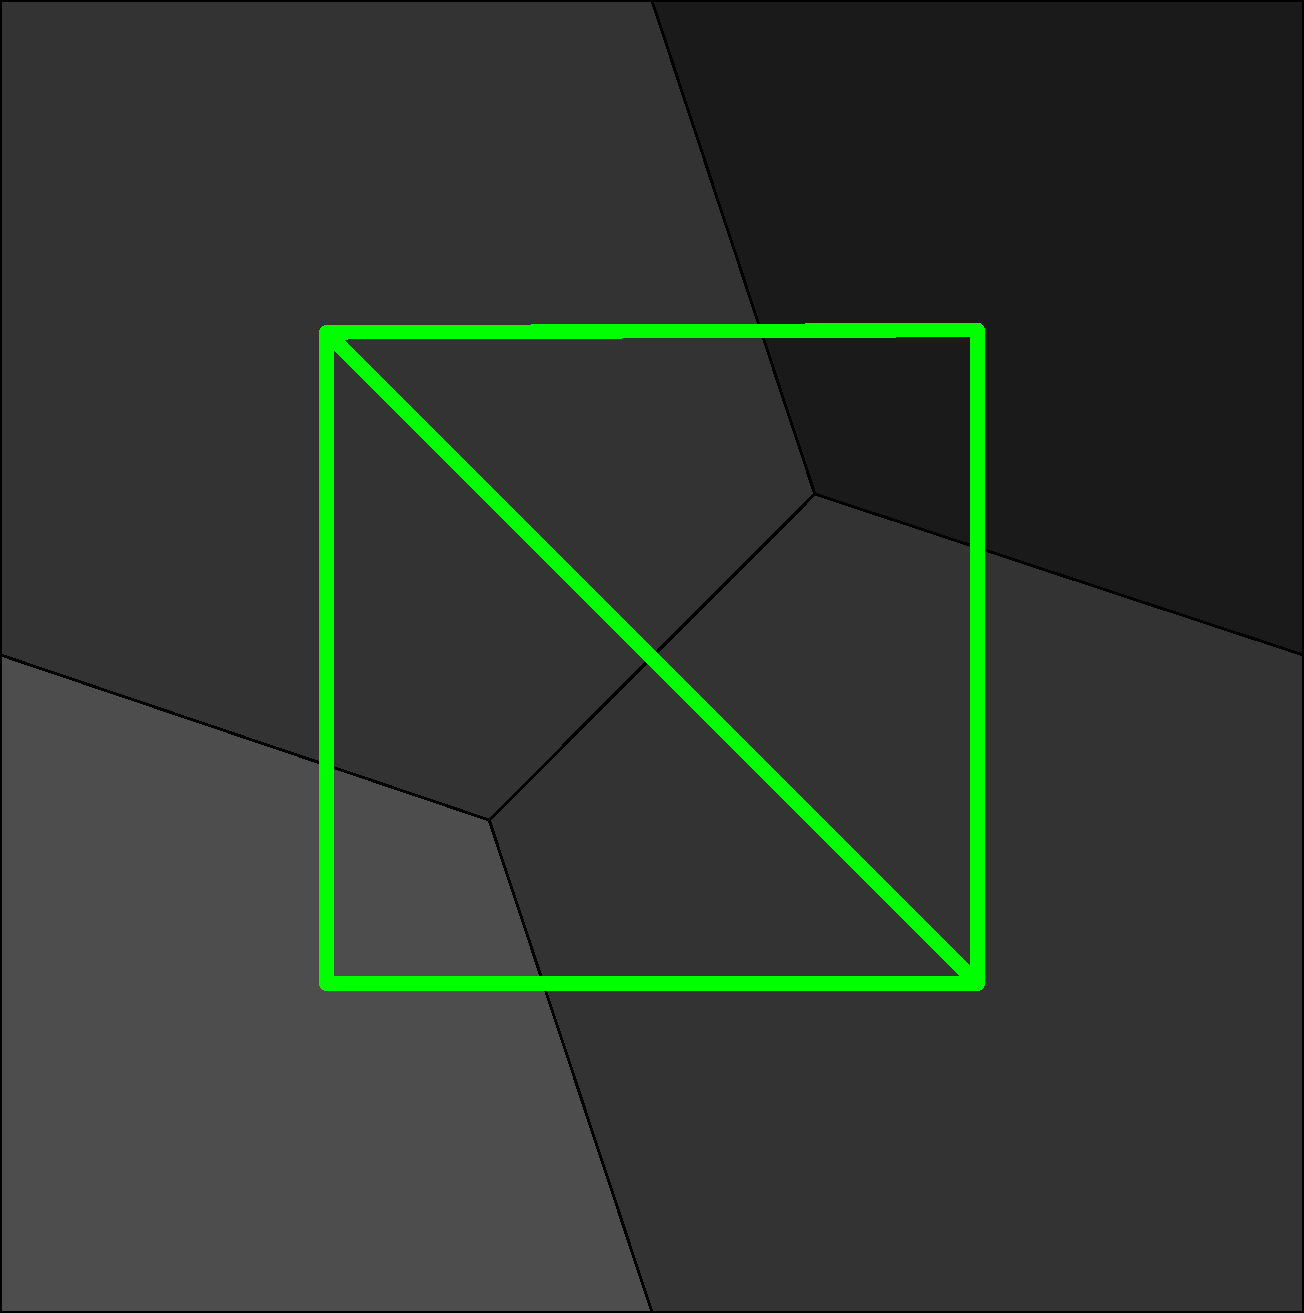
\includegraphics[width=0.8\textwidth]{assets/evil_pattern2.pdf}
  \caption{An evil pattern. A green line represents a connection (based on the
    similarity graph). The conversion to a Voronoi diagram based on the rules
    described in this document was already done in this sample.}
\end{figure}

The original Kopf-Lischinski paper describes fully connected graphs with
redundant crossing connections. The approach was to remove the redundant
crossing connections.

The existence of crossing connections prevents the conversion of the pixel graph
to Voronoi diagrams and all of them must be erased. This behaviour is kept here.

The original Kopf-Lischinski paper considers some crossing connections as
redundant, because no extra care was taken to preserve more color information,
but the \emph{evil pattern \#2} requires an extra rule to produce better
results. We handle these nodes by \textbf{NOT} removing the diagonal connection
and handling them with the heuristics for \hyperref[white_nodes]{white nodes}.

There is, however, an extra step that replaces the ``\emph{remove safe and
redundant crossing connections}'' step described in the original Kopf-Lischinski
paper. The new algorithm should detect if only one of the crossing connections
glue nodes of equal colors (as opposed to similar colors) and preserve it over
the other connection. If the detection fails, just fallback to the old
Kopf-Lischinski technique. We'll handle the new nodes using the same rules for
\hyperref[white_nodes]{white nodes}. Note that this new rule is \textbf{not} a
classic heuristic that will compete with the other heuristics (islands, sparse
pixels, \ldots{}).

This approach is an improvement, because it'll favor a pattern where cells that
share the same color will share an edge. Thus, they will be summed together in
the same polygon in later processing steps, creating splines that are more
smooth, natural and can be optimized more easily.

\subsection{The evil pattern \#3}

An example of the \emph{evil pattern \#3} follows:

\begin{figure}[H]
  \centering
  
\includegraphics[width=0.8\textwidth]{assets/evil_pattern3.pdf}
  \caption{An evil pattern. A green line represents a connection (based on the
    similarity graph). The colors of the nodes on the main diagonal are the
    same.}
\end{figure}

The \emph{evil pattern \#3} is resolved by the technique developed to handle the
\hyperref[evil_pattern2]{evil pattern \#2}. If only one of the two connections
share the \textbf{same} color, then this should be the connection preserved.

\subsection{Other evil patterns}

There are other the evil patterns (the evil pattern \#3, where the colors of the
main diagonal are different, for instance). I give up here.

The new rules are added as an extra step on the process. They are not treated
like the Kopf-Lischinski's heuristics to resolve crossing connections. I think
maybe would be possible to get some of the new rules and describe versions that
are more general and can be added to the "container" that holds the old
heuristics. To make this happen, I'd need to define the concept of "similar
color" as a set and operations on top of the set, the notion of interval and
other things and logical reasoning on top of all that. A bit of mathematical
work to improve the quality a little more, but I wanna to investigate the use of
La*b* colors (an old suggestion by Nathan) to replace the current concept of
"similar colors". I didn't replaced the current space color until now, because
YUV and La*b* behave differently and I couldn't just convert the YUV constants
that define the boundary between dissimilar colors to La*b* to achieve better
results. The current YUV constants were taken from HQx filter and I need to
define a methodology to find new constants.

The advantage of a rule that is more general and unifies behaviour is just the
beauty of a simpler rule that handles the real problem, as opposed to several
branches that are consequence of the real problem. It'd abstract the nature of
the problem better. It'd make the code simpler. It'd handle more branches. Being
a single rule that affect more branches, it'd be easier to test and better at
convincing me that the improvement is real and there will be no loss of quality
in other images.

It'd be interesting to investigate the range of voting in all heuristics and try
to come up with "fair" multipliers/strength.
